\documentclass[a4paper,12pt]{article} 
\usepackage[T1]{fontenc}              
\usepackage[frenchb]{babel} % césures, titres français
\usepackage[utf8]{inputenc} % encodage
\usepackage[a4paper,left=3cm,right=3cm,top=2cm,bottom=2cm]{geometry} % marges
\usepackage{graphicx} % insertion d'images
\usepackage{rotating}
\usepackage{float} % permet d'utiliser H pour placer un flottant obligatoirement
\usepackage{pdfpages} % inclusion de PDF au sein du document
\usepackage{listings}
\pagestyle{plain} % pied de pages simples

\setlength{\parskip}{1ex plus 0.5ex minus 0.2ex} % espace entre les paragraphes
\setcounter{tocdepth}{2}
\setcounter{secnumdepth}{2}

\lstset{% general command to set parameter(s)
basicstyle=\ttfamily, % print whole listing small
keywordstyle=\color{black}\bfseries\underbar,
% underlined bold black keywords
identifierstyle=, % nothing happens
commentstyle=\color{white}, % white comments
showstringspaces=false,
numbers=left,
language=java,
breaklines=true,
frame=tblr} % no special string spaces

%%%% debut macro %%%%
\makeatletter
\renewcommand\section{\@startsection {section}{1}{\z@}%
                           {-3.5ex \@plus -1ex \@minus -.2ex}%
                           {2.3ex \@plus.2ex}%
                           {\normalfont\Large\bfseries}}
\makeatother
%%%% fin macro %%%%



% Def
\newcommand{\code}[1]{{\lstinline{#1}}}

\begin{document}
\newpage
\title{J2EE\\TP1}
\date{}
\author{BRIZAI Olivier\\THORAVAL Maxime}
\maketitle

\newpage
Le but de ce TP était de réaliser une application simple dans le but d'apprendre et comprendre la configuration d'un serveur Tomcat.

\section{Fonctionnement de l'application}
Notre application est simpliste et n'est que peu modifiée par rapport à ce qui était demandé dans le sujet.

\begin{figure}[H]
	\center
	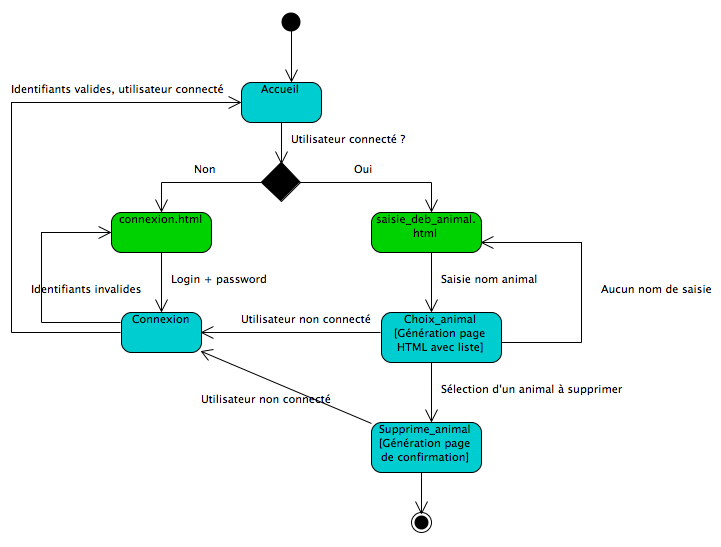
\includegraphics[width=15cm]{diag.png}
	\caption{Fonctionnement de notre application}
\end{figure}

Dans un premier temps, l'utilisateur arrive sur une servlet d'accueil, celle-ci vérifie s'il est connecté. Si non, il est dirigé vers le formulaire de connexion, si oui, vers le formulaire de saisie de nom d'animal. Pour se connecter, l'utilisateur doit rentrer un login et un mot de passe, si ceux-ci sont faux, il reste sur la même page, s'ils sont valides, il est redirigé vers la servlet d'accueil (et va pouvoir saisir le nom d'animal). Une fois le nom saisie, celui-ci est transmis à une servlet (\textit{Choix\_animal}) qui va s'occuper de récupérer tous les animaux, contenant l'information entrée, et générer une liste déroulante. L'utilisateur sélectionne l'animal souhaité et clique sur \og Supprimer \fg. Ce choix est transmis à une autre servlet (\textit{Supprime\_animal}), qui va elle se charger d'effectuer la suppression au sein de la base de données. Pour les deux dernières servlets, il y a systématiquement vérification de la session de l'utilisateur.

Nous avons une classe supplémentaire (\textit{GestionBDD}) qui fait l'interface entre les servlets et la base de données.

\section{web.xml}
Voyons maintenant quelques bribes de notre fichier \textit{web.xml}.


Nous définissons ainsi les applets et leur donnons un nom.
\begin{lstlisting}
	<servlet>
		<description>
		</description>
		<display-name>Connexion</display-name>
		<servlet-name>Connexion</servlet-name>
		<servlet-class>
		clinique.Connexion</servlet-class>
	</servlet>
	<servlet>
		<description>
		</description>
		<display-name>Accueil</display-name>
		<servlet-name>Accueil</servlet-name>
		<servlet-class>
		clinique.Accueil</servlet-class>
	</servlet>
\end{lstlisting}
Nous pouvons maintenant \og mapper \fg{} (relier) ces servlet (à l'aide de leur nom) à une url.
\begin{lstlisting}
<servlet-mapping>
	<servlet-name>Connexion</servlet-name>
	<url-pattern>/Connexion</url-pattern>
</servlet-mapping>
<servlet-mapping>
	<servlet-name>Accueil</servlet-name>
	<url-pattern>/Accueil</url-pattern>
</servlet-mapping>
\end{lstlisting}
Pour finir, nous déclarons la servlet \textit{Accueil} comme page d'index (page appelée par défaut lorsqu'aucune n'est renseignée).
\begin{lstlisting}
<welcome-file-list>
	<welcome-file>Accueil</welcome-file>
</welcome-file-list>
\end{lstlisting}


\section{Autres informations}
\subsubsection{Redirections}
Dans de nombreuses étapes de notre application, nous effectuons des redirections. Cela est possible grâce à cette fonction :
\begin{lstlisting}
response.sendRedirect("connexion.html");
\end{lstlisting}

\subsubsection{Utilisateurs}
Afin de gérer les utilisateurs, une table \textit{utilisateur} a été crée au sein de la base de données postgres. Elle ne contient que deux champs : login et password.


\end{document}


